\chapter{Десятичные дроби и проценты}\markright{Глава 4}
\begin{definition}\term{Десятичная дробь} (\emph{decimal}) — запись числа с разрядами десятых, сотых, тысячных и далее после запятой.\end{definition}
\begin{definition}\term{Процент} (\emph{percent}) — одна сотая часть: \(1 \% = \frac{1}{100} = 0{,}01\).\end{definition}
\begin{definition}\term{Периодическая десятичная дробь} (\emph{repeating decimal}) — бесконечная десятичная дробь с повторяющимся блоком цифр начиная с некоторого разряда.\end{definition}
\section*{Правила вычислений}
При сложении и вычитании десятичных дробей записывай одинаковые разряды друг под другом.\par
При умножении сначала умножь без запятых, затем отдели справа столько цифр, сколько их было после запятых в обоих множителях вместе.\par
При делении перенеси запятую в делимом и делителе на одинаковое число разрядов, чтобы делитель стал целым.\par
\section*{Формулы для процентов}
\(p \%\) от \(A\): \(A \cdot \frac{p}{100}\). Если \(p \%\) числа равны \(B\) и \(p \ne  0\), то число равно \(\frac{100 B}{p}\).\par
Рост на \(p \%\): \(A (1 + \frac{p}{100})\). Снижение на \(p \%\): \(A (1 - \frac{p}{100})\).\par
Процентное изменение: \(\frac{\text{новое значение} - \text{старое значение}}{\text{старое значение}} \cdot 100 \%\), если старое значение не равно \(0\). В обычных задачах о цене исходная цена положительна.\par
Каждый следующий процент изменения относится к уже изменённой величине.\par
\section*{Округление и периодические дроби}
Если следующая за оставляемым разрядом цифра \(0 - 4\), разряд не меняют; если \(5 - 9\), увеличивают на \(1\), при необходимости перенося единицу в старший разряд.\par
Любая периодическая десятичная дробь представляет рациональное число.\par
{\small\textit{Пример: \(\frac{1}{3} = 0{,}(3)\). Цена \(100\) рублей после двух скидок по \(10 \%\): \(100 \cdot 0{,}9 \cdot 0{,}9 = 81\) рубль.}}\par
\Needspace{7\baselineskip}\section*{Задачи}
\begingroup\setlength{\parskip}{3pt}
\noindent\begin{minipage}[t]{\linewidth}\textbf{4.1.} Вычисли \(3{,}75 + 0{,}086\).\par\end{minipage}\par
\noindent\begin{minipage}[t]{\linewidth}\textbf{4.2.} Вычисли \(8 - 2{,}47\).\par\end{minipage}\par
\noindent\begin{minipage}[t]{\linewidth}\textbf{4.3.} Вычисли \(0{,}24 \cdot  0{,}5\).\par\end{minipage}\par
\noindent\begin{minipage}[t]{\linewidth}\textbf{4.4.} Вычисли \(4{,}2 : 0{,}07\).\par\end{minipage}\par
\noindent\begin{minipage}[t]{\linewidth}\textbf{4.5.} Запиши \(\dfrac{7}{8}\) десятичной дробью.\par\end{minipage}\par
\par\addvspace{5pt}\begin{lrbox}{\CatFlowBox}\begin{minipage}[t]{\linewidth}
\setlength{\parskip}{5pt}\setlength{\columnsep}{4.5mm}\setlength{\intextsep}{0pt}
\begin{wrapfigure}[9]{l}{54mm}

\includegraphics[width=54mm,height=58mm,keepaspectratio]{images/unique/art-14.png}
\end{wrapfigure}
\textbf{4.6.} Запиши \(0{,}125\) несократимой обыкновенной дробью.\par

\textbf{4.7.} Запиши \(\dfrac{2}{3}\) периодической десятичной дробью.\par

\textbf{4.8.} Округли \(3{,}14159\) до сотых и до тысячных.\par

\textbf{4.9.} Найди \(15 \%\) от \(240\).\par

\textbf{4.10.} \(30 \%\) числа равны \(54\). Найди число.\par

\textbf{4.11.} Цена выросла с \(800\) до \(920\) рублей. На сколько процентов?\par

\textbf{4.12.} Цену \(1000\) рублей повысили на \(20 \%\), затем снизили на \(20 \%\). Найди итоговую цену и изменение в процентах от исходной.\par
\par\WFclear\end{minipage}\end{lrbox}%
\ifdim\dimexpr\ht\CatFlowBox+\dp\CatFlowBox\relax<64mm\dp\CatFlowBox=\dimexpr64mm-\ht\CatFlowBox\relax\fi%
\noindent\usebox{\CatFlowBox}\par\addvspace{5pt}

\noindent\begin{minipage}[t]{\linewidth}\textbf{4.13.} Купили \(1{,}8\) кг яблок по \(125\) рублей за килограмм. Сколько заплатили?\par\end{minipage}\par
\noindent\begin{minipage}[t]{\linewidth}\textbf{4.14.} Куртка стоит \(4800\) рублей. Скидка составляет \(15 \%\). Какова цена со скидкой?\par\end{minipage}\par
\noindent\begin{minipage}[t]{\linewidth}\textbf{4.15.} Велосипедист проехал \(7{,}86\) км утром и \(5{,}47\) км вечером. Найди общий путь и округли его до десятых километра.\par\end{minipage}\par
\noindent\begin{minipage}[t]{\linewidth}\textbf{4.16.}\starmark{} После скидки \(20 \%\) и следующей скидки \(10 \%\) товар стоит \(2160\) рублей. Найди исходную цену.\par\end{minipage}\par
\noindent\begin{minipage}[t]{\linewidth}\textbf{4.17.}\starmark{} Цена выросла на \(25 \%\). На сколько процентов нужно снизить новую цену, чтобы получить исходную?\par\end{minipage}\par
\noindent\begin{minipage}[t]{\linewidth}\textbf{4.18.}\starmark{} Смешали \(200\) г раствора с массовой долей соли \(10 \%\) и \(300\) г раствора с долей соли \(20 \%\). Найди массовую долю соли в смеси.\begin{center}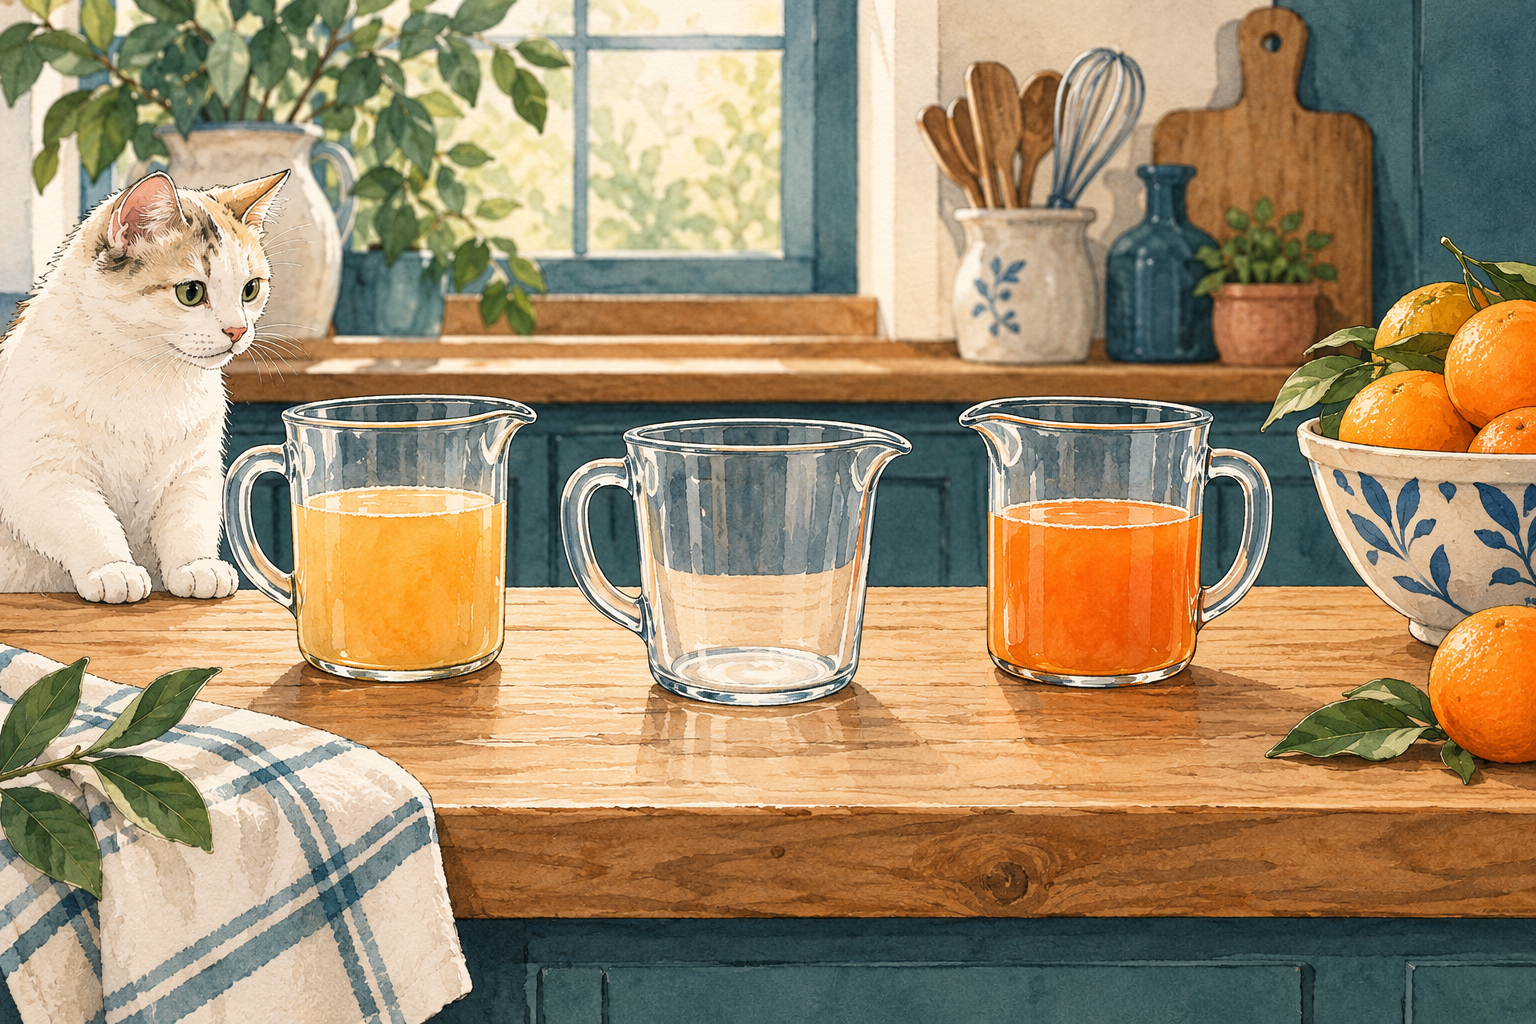
\includegraphics[width=.7\linewidth,height=45mm,keepaspectratio]{images/cats-mixtures.png}\end{center}\par\end{minipage}\par
\noindent\begin{minipage}[t]{\linewidth}\textbf{4.19.} Положительная цена сначала выросла на \(p\%\), затем новая цена выросла на \(q\%\), где \(p,q\ge0\). Докажи, что общее увеличение составляет \(\left(p+q+\dfrac{pq}{100}\right)\%\) от исходной цены.\par\end{minipage}\par
\noindent\begin{minipage}[t]{\linewidth}\textbf{4.20.}\starmark{} Пусть \(\dfrac pq\) --- положительная несократимая дробь с целыми \(p,q>0\). Докажи, что она имеет конечную десятичную запись тогда и только тогда, когда \(q=2^{\alpha}5^{\beta}\) для некоторых \(\alpha,\beta\in\mathbb N_0\). Можно пользоваться основной теоремой арифметики и свойствами делимости.\par\end{minipage}\par
\endgroup
